\chapter{Surface Reconstruction}
\label{appx:AltSurfRecon}
\todourgent[inline,author=Benni]{@ JuanCarlos: refer to this section in future work}
Our implementation of the surface reconstruction scheme (see \autoref{ssec:reconstruction}) and the two-scale approach (see \autoref{ssec:parametrization}) so far only allows simple structures like spheres or tori if one is restricted to few NURBS patches. For more complicated structures -- for example the output of a topology optimization tool -- we currently have to use a very high resolution, which results in very costly calculations. An alternative approach is the application of a more elaborate surface extraction scheme. A short summary of different schemes is given in the following.

\section{Manifold Dual Contouring}
Our implementation of \ac{DC} is a very basic one. This causes problems when it comes to the coarse resolution of our two scale approach: We need as coarse a mesh as possible, which has the same topology as our fine mesh. These goals cannot be reached with a basic approach, but only with an adaptive and topology safe \ac{DC} algorithm like \emph{Manifold Dual Contouring} \cite{Schaefer2007}.

\section{Dual Marching Methods}
The non-manifold edges generated by \ac{DC} have been resolved by applying a remeshing scheme. But there are also hybrid methods of \ac{DC} and \ac{MC}, which have been developed to cope with the drawbacks of each. These methods use ideas from both the \ac{MC} and the \ac{DC} approaches. Using one of these methods would be a way of inherently avoiding non-manifold edges while keeping all the beneficial properties of \ac{DC}. Here, we briefly introduce two of those hybrid methods:
\begin{itemize}
\item \textbf{\acl{DualMC}:}
The \acf{DualMC} method is a hybrid of \ac{MC} and \ac{DC}: We traverse the cubes like in \ac{MC} and insert vertices and connect them like in \ac{DC}. The combination of the $256$ different cases from the basic \ac{MC}, the extension for creating non-ambiguous surfaces, and the framework of \ac{DC} -- these result in a very effective but also complex algorithm. A drawback of this method is that for certain configurations it ends up creating non-\ac{quad} faces. We refer the interested reader to  \cite{Nielson2004, Zhang2012,ScottSchaefer2004}.

\item \textbf{\acl{DualMT}:}
While \ac{DualMC} is a very complicated algorithm, \acf{DualMT} uses tetrahedra instead of cubes and therefore reduces the $256$ different cases from \ac{MC} to $2^4=16$ cases. Furthermore, a treatment of ambiguous cases is not necessary anymore since there are no ambiguous cases for this method\todointern{really? check this or find reference!}.
Even though the method is working on tetrahedra, we can still apply it to a voxel dataset, by composing each cube out of 5 or 6 tetrahedra (\autoref{fig:splittingCubes}). Nevertheless, this high amount of simplification comes with a drawback: the treatment of ambiguous cases depends on the splitting scheme applied to a cube\todointern{proof or reference! Show 2D example.}. Further details on this method can be found in \cite{Nielson2008}.

\end{itemize}

\begin{figure}
\begin{center}
\begin{subfigure}[t]{.45\textwidth}
\begin{center}
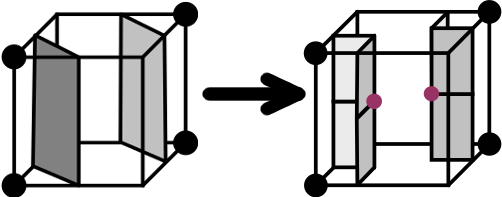
\includegraphics[width = .8\textwidth]{Pictures/SurfaceReconstruction/MCtoDualMC.png}
\subcaption{Treatment of one of the \ac{MC} cases in \ac{DualMC} algorithm (figure from \cite{Nielson2004})}
\end{center}
\end{subfigure}
\hfill
\begin{subfigure}[t]{.45\textwidth}
\begin{center}
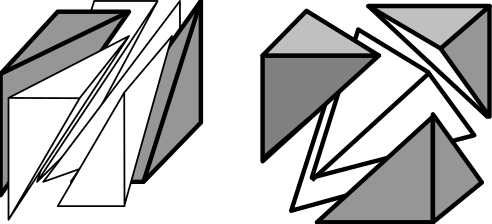
\includegraphics[width = .8\textwidth]{Pictures/SurfaceReconstruction/SplittingCubes.png}
\caption{Two different schemes for subdivision of cubes into tetrahedra (figure from \cite{Nielson2008})}
\label{fig:splittingCubes}
\end{center}
\end{subfigure}
\caption{Illustrations of Dual Marching methods.}
\end{center}
\end{figure}

\section{Cubical Marching Squares}
Another promising, yet not perfectly fitting method is the \emph{Cubical Marching Squares} method. Here one unfolds each cube and first investigates  its six faces. On the faces one determines the necessary edges and finally the region inside the cube, that is defined by the edges,  is polygonized (see \autoref{fig:CMS}). The main drawback of this method is that it only produces surfaces composed of triangular faces. Still it might be possible to modify this algorithm in a way that it outputs surfaces of quadrilateral faces. For detailed information we again recommend the original paper \cite{Ho2005}.

\begin{figure}
\begin{center}
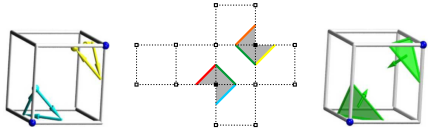
\includegraphics[scale=1]{Pictures/CMS.png}
\caption{Illustration of the unfolding technique applied in \emph{Cubical Marching Squares} from \cite{Ho2005}}
\label{fig:CMS}
\end{center}
\end{figure}
